\section{Auswertung}
\label{sec:Auswertung}
\subsection{Graphische Visualisierung}
\begin{figure}
  \centering
  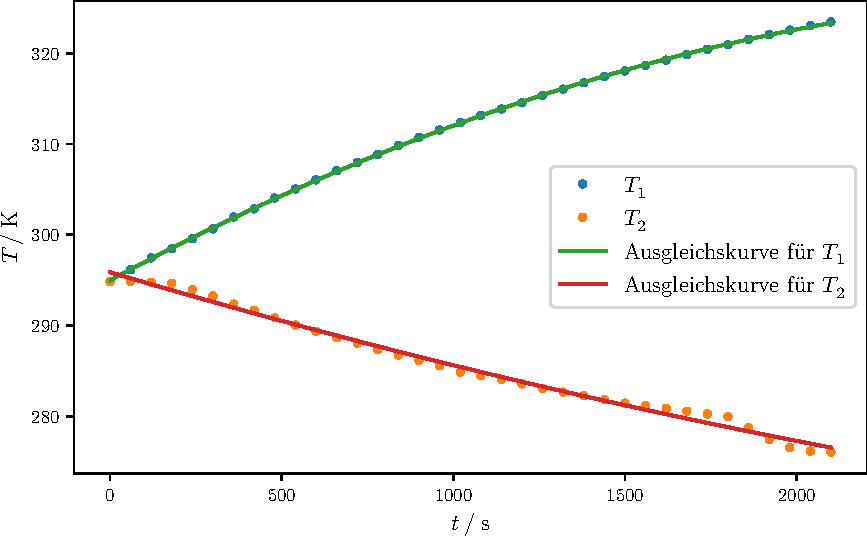
\includegraphics{temperatur.pdf}
  \caption{Temperaturverlauf beider Reservoirs.}
  \label{fig:temperatur}
\end{figure}
\subsection{Nicht-lineare Ausgleichsrechnung}
Der nicht-lineare Zusammenhang zwischen der Zeit und der Temperatur lässt sich mittels einer quadtratischen Ausgleichskurve, welche durch 
\begin{equation}
  T(t) = At^2 + Bt + C
\end{equation}
beschrieben wird, approximieren. Mittels Rechnungen in Python ergaben sich die Ausgleichskfunktionen zu
\begin{align}
  T_1(t) &= - 0.0116t^2 + 1.2168 t + 294.7008 \\
  T_2(t) &= \phantom{-}  0.0034 t^2 - 0.6725 t + 295.8702
\end{align}
\subsection{Differentialquotient}
Die Differentialquotienten von $T_1(t)$ und $T_2(t)$ sind durch
\begin{align}
  \frac{\symup{d} T_1(t)}{\symup{d}t} = - 0.0232t + 1.2168  \\
  \frac{\symup{d} T_2(t)}{\symup{d}t} = \phantom{-} 0.0068 t - 0.6725 
\end{align}
gegeben. Die in die Differentialquotienten eingesetzen Zeitpunkte $t = 10$, $t = 15$, $t = 20$ und $t = 35$ ergeben folgende Tabelle:
\begin{table}
  \centering
  \caption{Ergebnisse der Differentialquotienten}
  \label{tab:TabelleDifferentialquotient}
  \sisetup{table-format = 1.4}
  \begin{tabular}{S[table-format = 2.0] S S}
    \toprule
    {$t \mathbin{/} \si{\second}$} & {$\frac{\symup{d} T_1(t)}{\symup{d}t} \mathbin{/} \si{\kelvin\second\tothe{-1}}$} & 
    {$\frac{\symup{d} T_2(t)}{\symup{d}t} \mathbin{/} \si{\kelvin\second\tothe{-1}}$} \\
    \midrule
    600  & 0.0164 &-0.0101 \\
    900  & 0,0145 &-0.0095 \\
    1200 & 0.0125 &-0.0089 \\
    2400 & 0.0067 &-0.0072 \\
    \bottomrule
  \end{tabular}
\end{table}
\subsection{Güteziffer}
Um die reale Güteziffer zu bestimmen dient die Gleichung \eqref{eqn:Güteziffer}.
Für die Wärmekapazität des Wassers gilt $m_1 c_\text{w}(T) = \SI{4}{\kilo\gram}\cdot c_\text{w}(T)$,
für die der Kupferschlangen $m_\text{k}c_\text{k} = \SI{750} {\joule\per\kelvin}$. Um die Genauigkeit der Rechnung zu erhöhen wurde hier die Temperaturabhängigkeit
der spezifischen Wärmekapazität $c_\text{w}(T)$ von Wasser berücksichtigt. Für die Berechnung der idealen Güterziffer $\nu_\text{id}$ ist die Beziehung \eqref{eqn:Id} von Nutzen.
Mittels Rechnungen ergaben sich die Werte der Güterziffern zu:
\begin{table}
  \centering
  \caption{Vergleich $\nu_\text{re}$ zu $\nu_\text{id}$}
  \label{tab:TabelleDifferentialquotient}
  \sisetup{table-format = 2.4}
  \begin{tabular}{S[table-format = 3.2] S[table-format = 1.4] S[table-format = 1.4] S S}
    \toprule
    {$T_1 \mathbin{/} \si{\kelvin}$} & {$ c_\text{w}(T_1) \mathbin{/} \si{\kilo\joule\kilo\tothe{-1}\gram\tothe{-1}\kelvin\tothe{-1}}$} & 
    {$\nu_\text{re}$} & {$\nu_\text{id}$} & {$\frac{\nu_\text{re}} {\nu_\text{id}} \si{\percent}$} \\
    \midrule
    306.05 & 4.1783 & 2.3866 & 18.3263 & 13.0230\\
    310.75 & 4.1783 & 2.1101 & 12.6321 & 16.7045\\    
    314.55 & 4.1787 & 1.8193 & 10.1468 & 17.9293\\  
    323.45 & 4.1807 & 0.9596 &  6.8238 & 14.0621\\    
    \bottomrule                                       
  \end{tabular}                                     
\end{table}\\
Während des Vergleichens beider Güteziffern wird auffällig, dass das Verhältnis sehr niedrig, im Bereich von $10$ bis $\SI{20}{\percent}$, liegt.
In der Gleichung \eqref{eqn:redWärm} wird gefordert, dass der Prozess der Wärmeübertragung ein reversibler Prozess ist,
und somit jede Energie, welche kurzfristig verloren geht, zurückgewonnen werden kann. Doch in der Realität ist diese nicht mehr 
zurück zu gewinnen. Beispielsweise kann die Energie in Form von Wärmeenergie an die Umwelt abgegeben werden.
